\section{Apps Similares}
\label{sec:Apps Similares}

    Examinar el mercado de software actual permitió delimitar los patrones de diseño consolidados y constatar qué carencias sufren los usuarios en su día a día. Existen herramientas consolidadas para cada fase por separado, pero ninguna cubre el recorrido completo. Se seleccionaron cinco plataformas representativas: portales de captación inmobiliaria generalista como Idealista~\cite{idealista}, servicios de alojamiento temporal como Airbnb~\cite{airbnb}, redes de alquiler por habitaciones como Badi~\cite{badi}, gestores contables como Tricount~\cite{tricount} y organizadores de tareas domésticas como Flatastic~\cite{flatastic}.

    Idealista~\cite{idealista} (figura~\ref{subfig:idealista}) domina el mercado inmobiliario en España gracias a su catálogo masivo y a un motor de búsqueda geográfica ágil. Su modelo de negocio se limita a la intermediación publicitaria inicial. El portal se desentiende por completo una vez establecido el contacto entre anunciante e interesado: no custodia fianzas, no verifica identidades mediante contratos formales y carece de herramientas para organizar la vida comunitaria tras la entrega de llaves.

    Airbnb~\cite{airbnb} (figura~\ref{subfig:airbnb}) dispone de una pasarela de pagos consolidada, gestión de depósitos en garantía y verificación de identidades mediante valoraciones recíprocas. Sin embargo, su orientación es turística. Las comisiones por servicio resultan prohibitivas para alquileres residenciales de media y larga duración. Tampoco contempla dinámicas de convivencia entre compañeros que comparten un mismo piso durante meses, delegando cualquier acuerdo interno a la comunicación informal externa.

    Badi~\cite{badi} (figura~\ref{subfig:badi}) nació orientada al alquiler de habitaciones en grandes núcleos urbanos, filtrando cuartos libres y perfiles de candidatos mediante un chat integrado. Pese a coincidir con la fase de captación de Colivi, su utilidad concluye con el acuerdo de entrada. La aplicación no acompaña a los inquilinos en el día a día: queda fuera cualquier herramienta para auditar gastos compartidos, coordinar la limpieza o dirimir desacuerdos domésticos.

    Tricount~\cite{tricount} (figura~\ref{subfig:tricount}) resuelve con solvencia el reparto de gastos mediante la simplificación de grafos de deuda entre múltiples participantes. Funciona como una libreta contable aislada. Carece de contexto inmobiliario real: los compañeros deben introducir cada concepto a mano sin vincularlo a contratos de alquiler, recibos oficiales o depósitos de fianza gestionados de forma conjunta con el propietario.

\begin{figure}[htbp]
    \centering
    \begin{subfigure}[b]{0.49\textwidth}
        \centering
        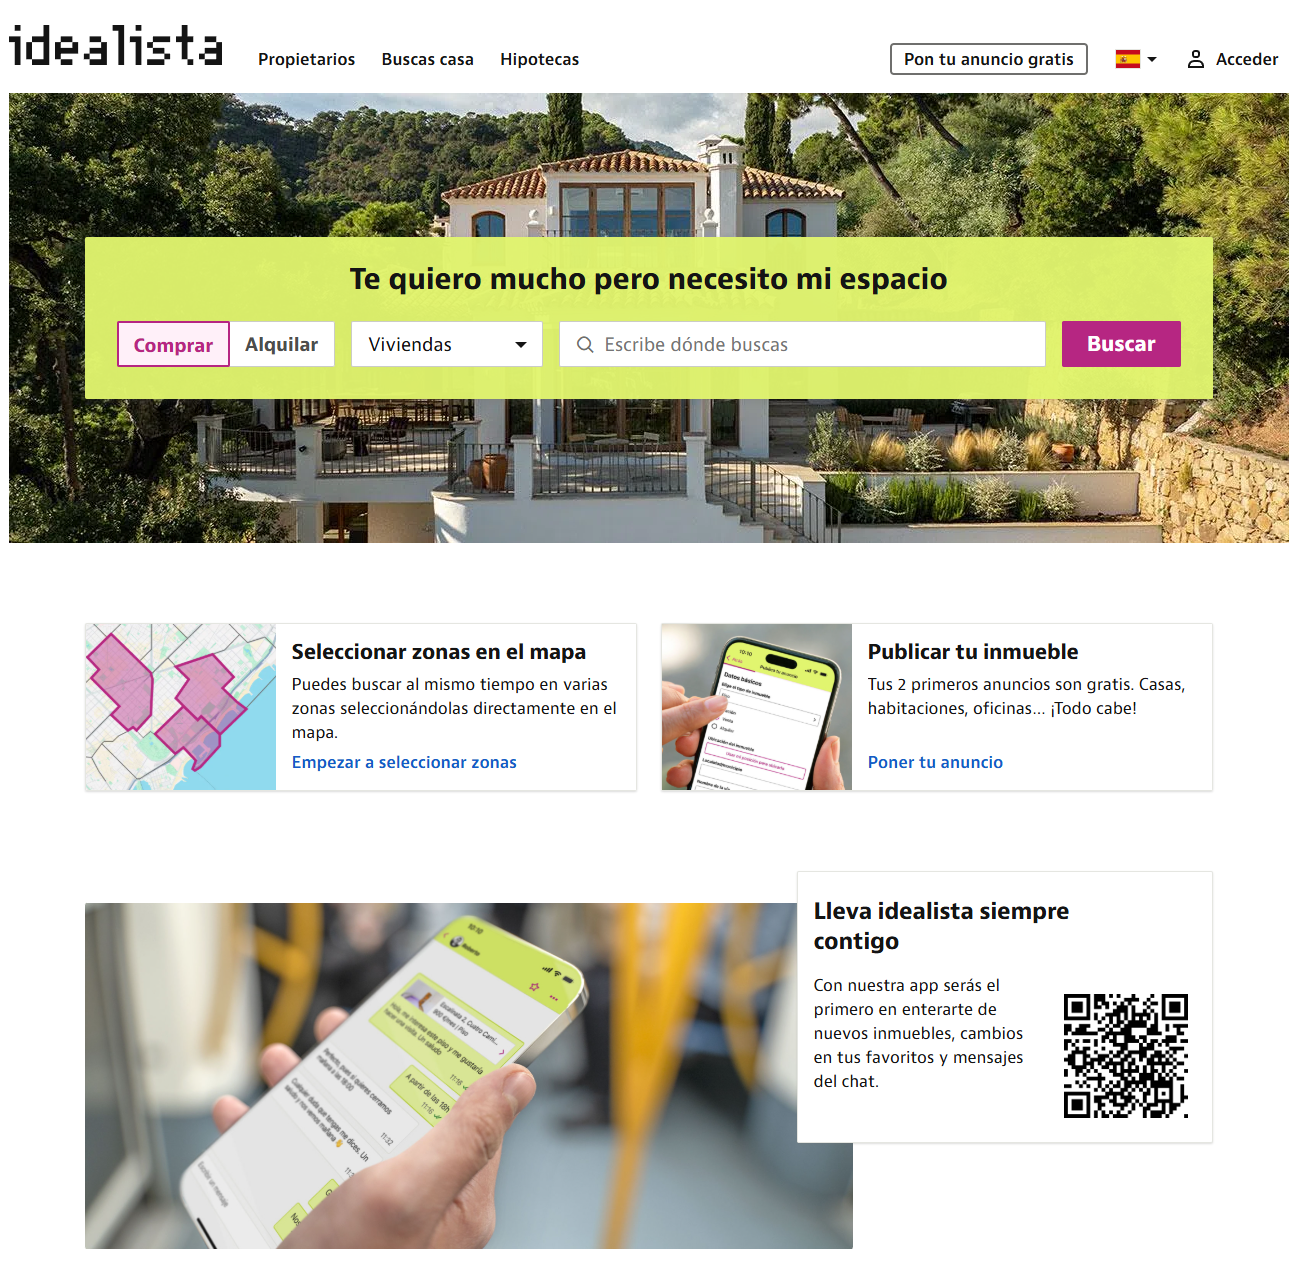
\includegraphics[width=\linewidth,height=7.8cm,keepaspectratio]{Introduccion/img/Idealista.png}
        \caption{Búsqueda en Idealista}
        \label{subfig:idealista}
    \end{subfigure}
    \hfill
    \begin{subfigure}[b]{0.49\textwidth}
        \centering
        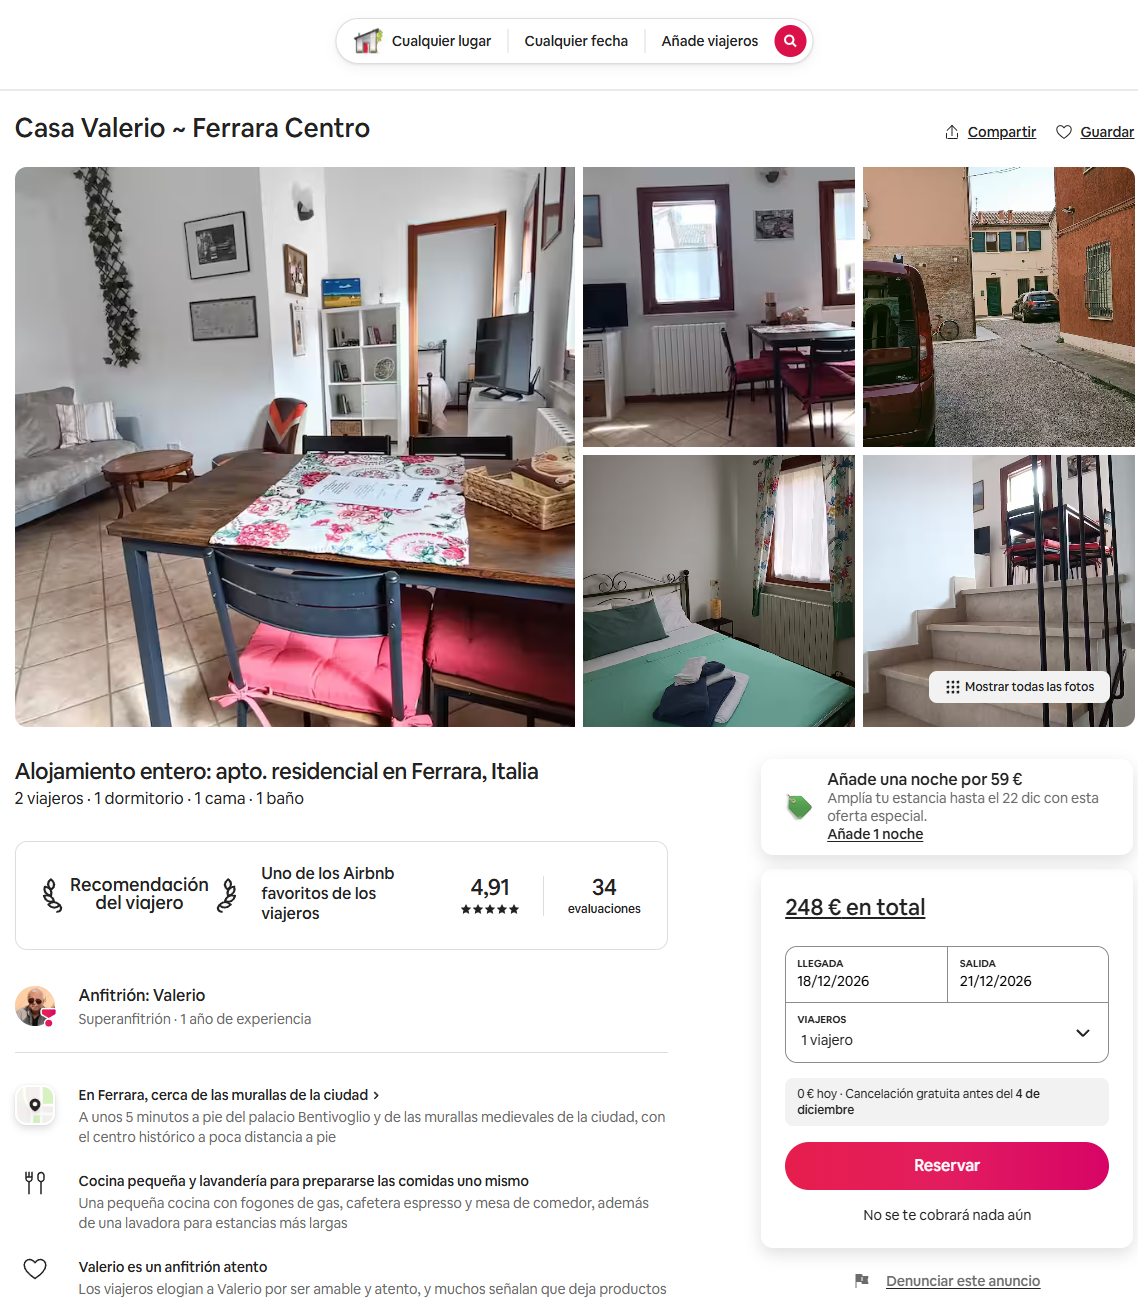
\includegraphics[width=\linewidth,height=7.8cm,keepaspectratio]{Introduccion/img/Airbnb.png}
        \caption{Detalles y reserva en Airbnb}
        \label{subfig:airbnb}
    \end{subfigure}
    
    \vspace{0.4cm}
    
    \begin{subfigure}[b]{0.49\textwidth}
        \centering
        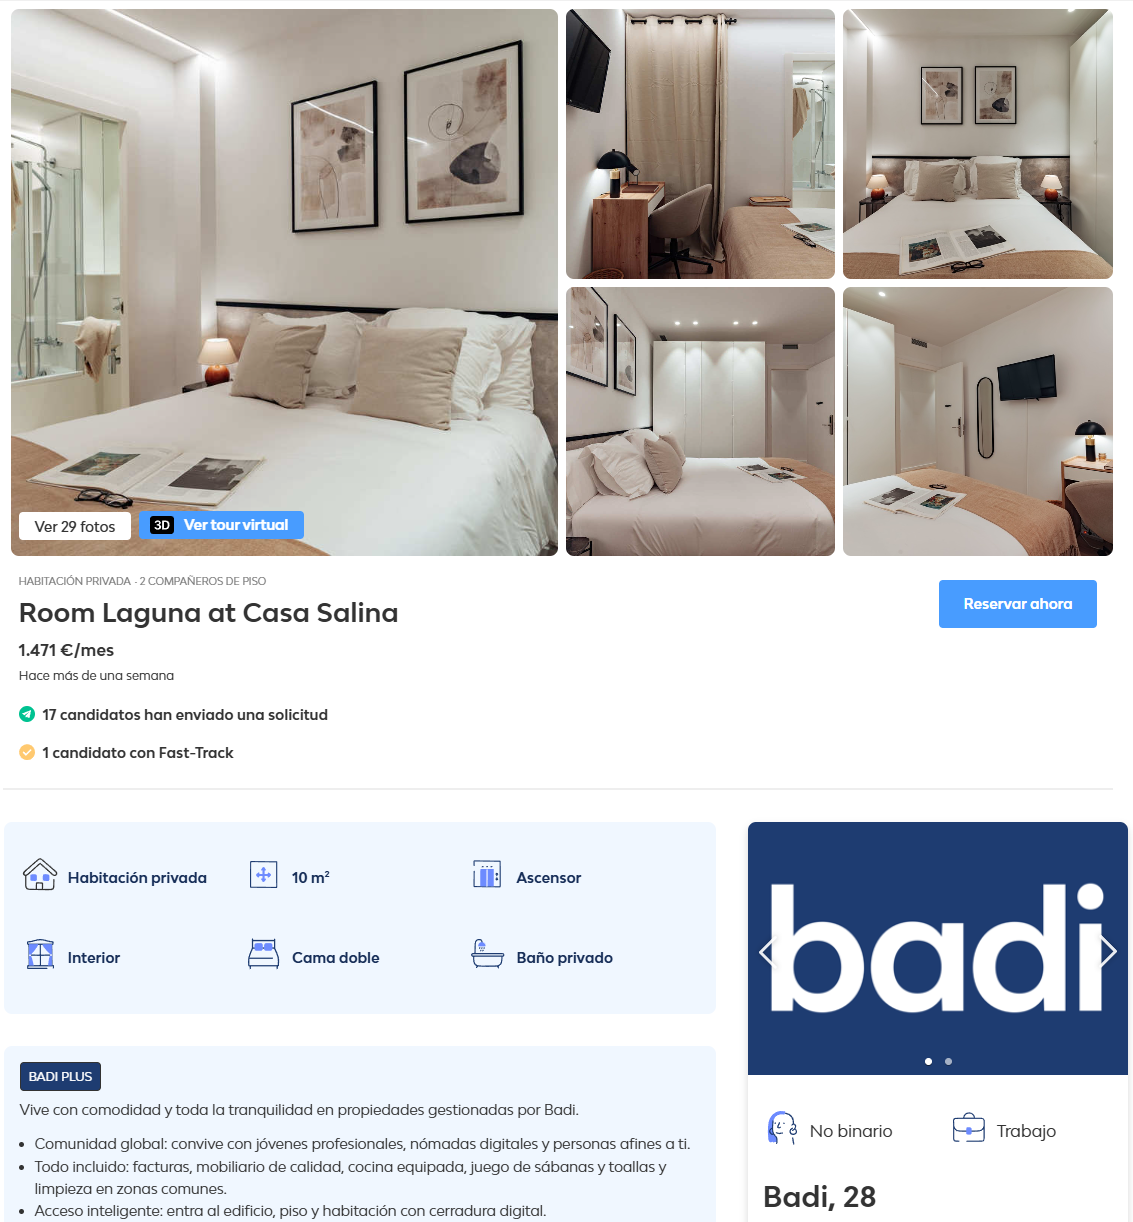
\includegraphics[width=\linewidth,height=7.8cm,keepaspectratio]{Introduccion/img/Badi.png}
        \caption{Habitaciones y perfiles en Badi}
        \label{subfig:badi}
    \end{subfigure}
    \hfill
    \begin{subfigure}[b]{0.49\textwidth}
        \centering
        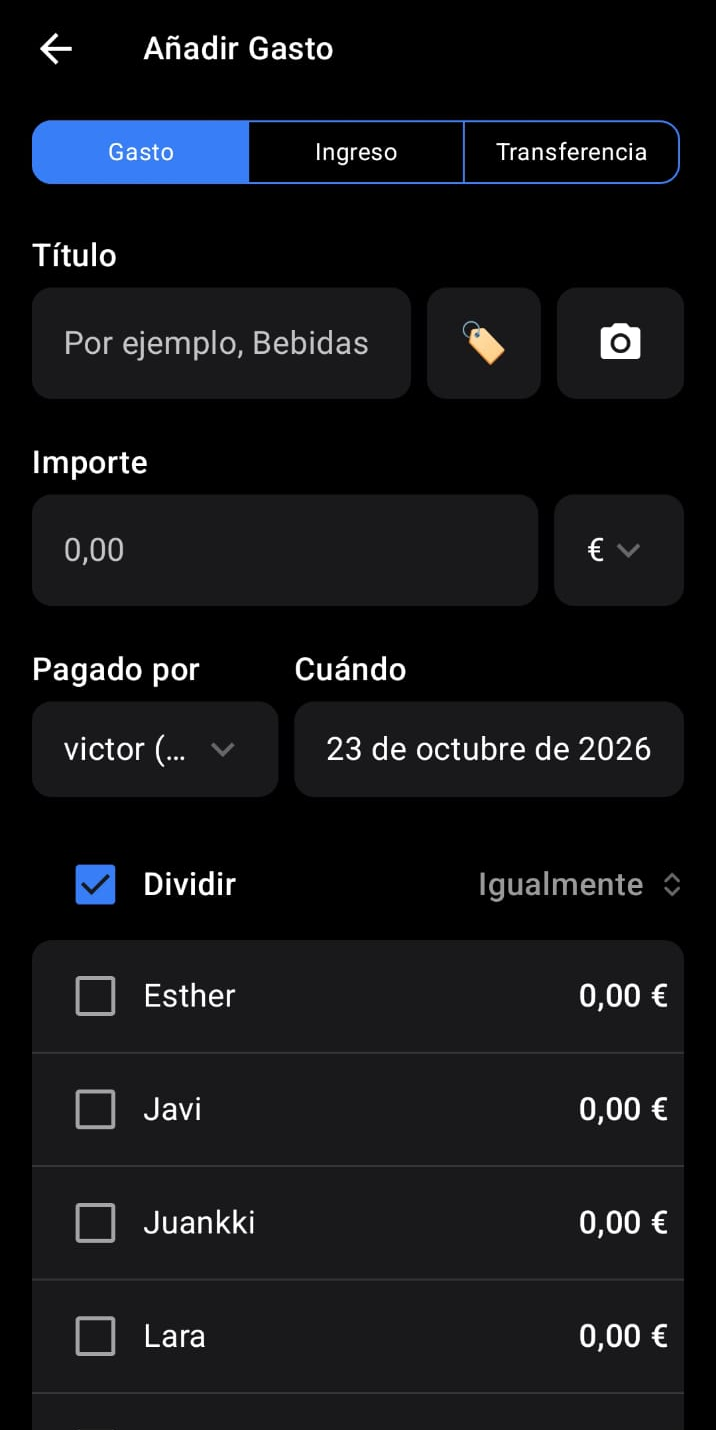
\includegraphics[width=\linewidth,height=7.8cm,keepaspectratio]{Introduccion/img/Tricount.png}
        \caption{Reparto de gastos en Tricount}
        \label{subfig:tricount}
    \end{subfigure}
    \caption{Interfaces de las principales soluciones analizadas en el mercado}
    \label{fig:apps_similares}
\end{figure}

    El ecosistema digital actual fragmenta la experiencia del inquilino en aplicaciones independientes sin conexión entre sí. Los usuarios buscan habitación en una web, firman el contrato en persona, anotan los gastos en una aplicación externa y discuten la limpieza por mensajería. Colivi unifica estas fases bajo una sola plataforma web y móvil, incorporando además un asistente basado en MCP para interactuar con los datos del hogar.

\begin{table}[htbp]
    \centering
    \caption{Comparativa de características entre plataformas analizadas y Colivi}
    \label{tab:comparativa_apps}
    \vspace{0.2cm}
    \resizebox{\textwidth}{!}{%
    \begin{tabular}{|l|c|c|c|c|c|c|}
        \hline
        \textbf{Plataforma} & \textbf{\begin{tabular}[c]{@{}c@{}}Catálogo y\\ Búsqueda\end{tabular}} & \textbf{\begin{tabular}[c]{@{}c@{}}Reserva y Fianza\\ Integrada\end{tabular}} & \textbf{\begin{tabular}[c]{@{}c@{}}Reparto de\\ Gastos Comunes\end{tabular}} & \textbf{\begin{tabular}[c]{@{}c@{}}Gamificación\\ de Tareas\end{tabular}} & \textbf{\begin{tabular}[c]{@{}c@{}}Asistente\\ IA (MCP)\end{tabular}} & \textbf{\begin{tabular}[c]{@{}c@{}}Enfoque\\ Coliving\end{tabular}} \\ \hline
        Idealista & Sí & No & No & No & No & No \\ \hline
        Airbnb & Sí & Sí & No & No & No & No \\ \hline
        Badi & Sí & No & No & No & No & Sí \\ \hline
        Tricount & No & No & Sí & No & No & No \\ \hline
        \textbf{Colivi (Propuesta)} & \textbf{Sí} & \textbf{Sí} & \textbf{Sí} & \textbf{Sí} & \textbf{Sí} & \textbf{Sí} \\ \hline
    \end{tabular}%
    }
\end{table}

    Las columnas de la tabla comparativa evalúan las siguientes capacidades técnicas y de dominio:

\begin{itemize}
    \item \textbf{Catálogo y Búsqueda}: motor público de localización con filtros espaciales, rangos de precio y comodidades del inmueble. Portales como Idealista, Airbnb y Badi satisfacen este criterio, mientras que utilidades contables como Tricount o Flatastic carecen de catálogo por definición.
    \item \textbf{Reserva y Fianza Integrada}: capacidad para formalizar acuerdos de estancia y retener o transferir depósitos de garantía mediante pasarelas auditables dentro del propio sistema. Solo Airbnb soporta este flujo en el mercado actual, pues Idealista y Badi delegan las transacciones económicas a pactos privados fuera de la plataforma.
    \item \textbf{Reparto de Gastos Comunes}: presencia de un motor de liquidación para prorratear facturas, calcular saldos individuales y registrar transferencias compensatorias. Supone el núcleo de Tricount, pero los portales de alquiler lo omiten en su totalidad.
    \item \textbf{Gamificación de Tareas}: mecanismos de rotación periódica del trabajo doméstico apoyados en asignaciones equitativas y tablas de clasificación. Únicamente Flatastic aproxima este concepto, aunque con métricas básicas sin trazabilidad inmutable del hogar.
    \item \textbf{Asistente IA (MCP)}: integración de un agente conversacional capaz de ejecutar herramientas sobre la base de datos del piso mediante el protocolo \emph{Model Context Protocol}. Ningún competidor del mercado incorpora agentes con acceso contextual al estado de tareas o finanzas de la vivienda.
    \item \textbf{Enfoque Coliving}: diseño centrado en el arrendamiento por habitaciones con zonas comunes y convivencia comunitaria entre estudiantes o jóvenes profesionales. Badi y Flatastic comparten esta orientación, diferenciándose de modelos turísticos o residenciales familiares.
\end{itemize}

Determinadas características exigen matices técnicos. Badi, por ejemplo, gestiona un cobro inicial para formalizar la reserva, pero no asume la custodia ni la restitución de la fianza durante la vigencia del contrato de arrendamiento. De igual forma, las opciones de atención automatizada en portales como Airbnb se limitan a centros de ayuda estáticos con preguntas frecuentes, sin conectividad hacia un servidor de contexto capaz de inspeccionar los registros internos del alojamiento.